\documentclass{standalone}
\usepackage{tikz}
\usetikzlibrary {angles,quotes,calc, positioning}
\begin{document}
    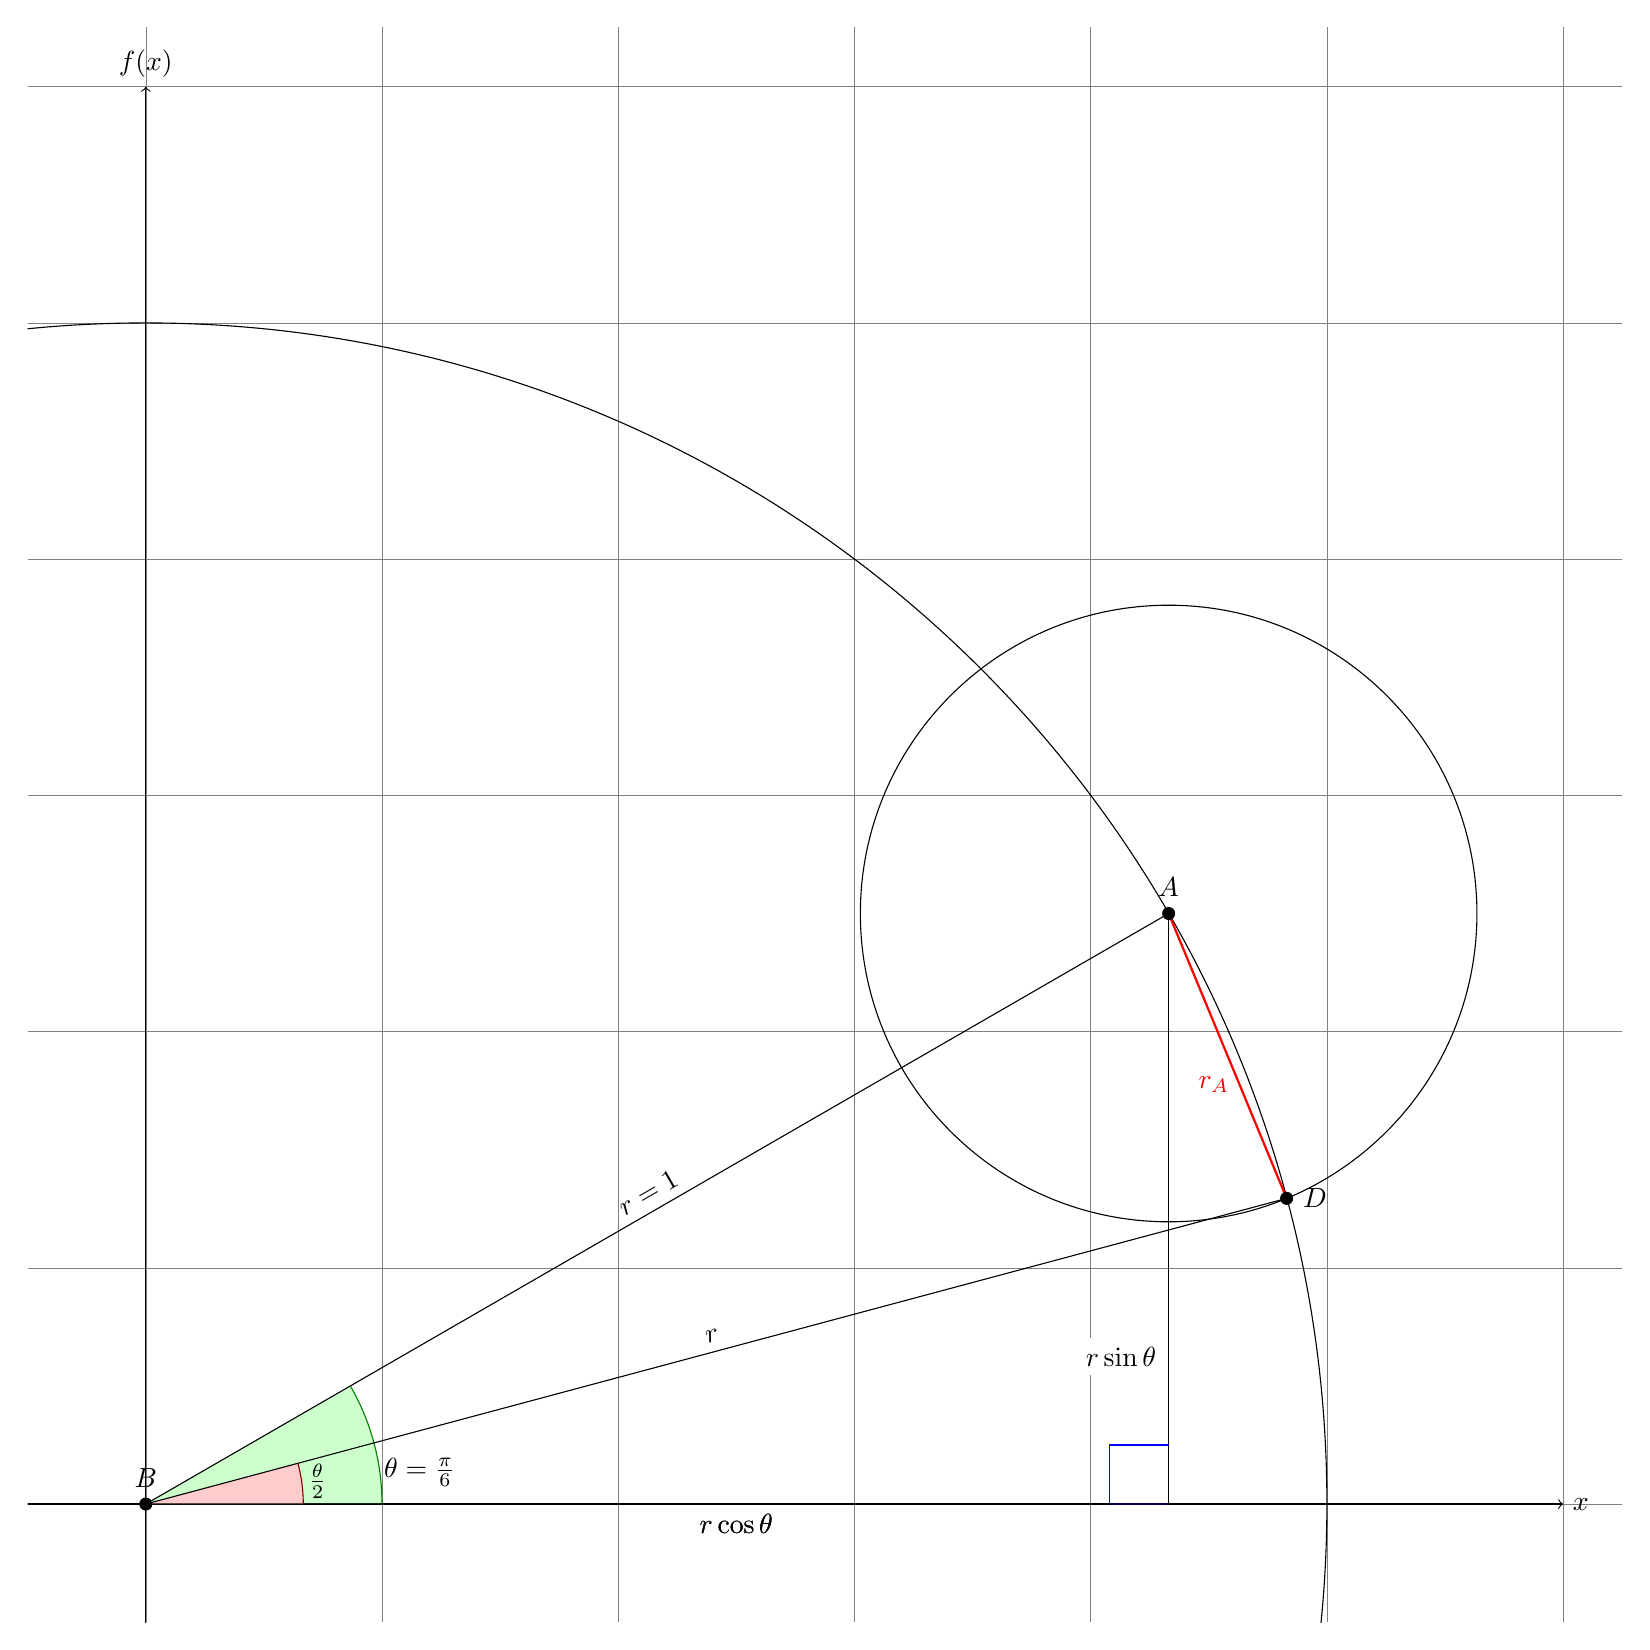
\begin{tikzpicture}[scale=15]

        % selecting the first quadrant
        \clip (-0.1,-0.1) rectangle (1.25,1.25);
        % setting up the Cartesian Grid. Note "help lines" = "gray, very thin"
        \draw[step=.2cm,help lines] (-.1,-.1) grid (2,2);
        % setting up the real and imaginary axis. 
        \draw[->] (-1.5,0) -- (1.2,0) coordinate (x axis) node[right] {$x$};
        \draw[->] (0,-1.5) -- (0,1.2) coordinate (y axis) node[above] {$f(x)$};


        \coordinate (A) at (30:1cm);
        \coordinate (B) at (0,0);
        \coordinate (G) at (1,0);
        \coordinate (D) at (15:1cm);

        \draw (B) circle [radius=1] node[circle,fill, scale=0.5, label=above:{$B$}] {};

        % project a line from A down to the x-axis
        \draw (A) -- node[left=1pt,fill=white, near end] {$r\sin \theta$} (A |- x axis);
      

        \draw (G) -- node[midway, below] {$r \cos \theta$} (B) -- node[midway, above, sloped] {$r=1$} (A)
              pic [draw=green!50!black, fill=green!20, angle radius=30mm, angle eccentricity = 1.2,
                   "$\theta=\frac{\pi}{6}$"{yshift=-15}] {angle = G--B--A};

        \draw [blue] (A |- x axis) -- ++(-.05,0) -- ++(0,.05) -- ++(.05,0); 
    
        % solution - to see the solution, uncomment out the comments, and recomment the lines directly after them
        %\draw[red, thick] (A) -- node[midway, right, text width=3cm, xshift=.55cm] {$2r|\sin\frac{\theta}{4}| = \sqrt{2-\sqrt{2+\sqrt{3}}}$ if $(r,\theta) = (1,\frac{\pi}{6}$)} (D);
        \draw[red, thick] (A) -- node[pos=.6, left] {$r_A$} (D);

        %\draw (A) circle [radius={2*sin(pi/24 r)}] node[circle,fill, scale=0.5, label=above:{$r\cos\theta,r\sin\theta$}] {};
        \draw (A) circle [radius={2*sin(pi/24 r)}] node[circle,fill, scale=0.5, label=above:{$A$}] {};

        \draw (G) -- node[midway, below] {$r \cos \theta$} (B) -- node[midway, above,sloped] {$r$} (D)
        pic [draw=red!50!black, fill=red!20, angle radius=20mm, angle eccentricity = 1.1, "$\frac{\theta}{2}$"] {angle = G--B--D};

        %\node[circle,fill,label=right:{$r\cos\frac{\theta}{2}, r\sin\frac{\theta}{2}$}, scale=0.5] at (D) {};
        \node[circle,fill,label=right:{$D$}, scale=0.5] at (D) {};

        %\node[circle,fill,label=left:{$r\cos\theta, r\sin\frac{\theta}{2}$}, scale=0.5] at ({cos(30)},{sin(15)}) (E) {};
        %\node[circle,fill,label=left:{$E$}, scale=0.5] at ({cos(30)},{sin(15)}) (E) {};

        % \draw (D)  -- (E) -- (A);



    \end{tikzpicture}
\end{document}
